% **************************************************************************************************
% **************************************************************************************************
\newsection{Floats: Graphics, Tables, and Listings}{intro:floats}



% **************************************************************************************************
\newsubsection{Figures and Tables}{intro:floats:figures}
Even relatively complex figures are easy to create, as you can see from this example. Note that you can refer to \Fref{fig:intro:floats:usage:figure}, but also to the subfigures: \Fref{fig:intro:floats:usage:figure-ex1} and \Fref{fig:intro:floats:usage:figure-ex2}.
\begin{figure}
  \centering
  \subfigure[left side]{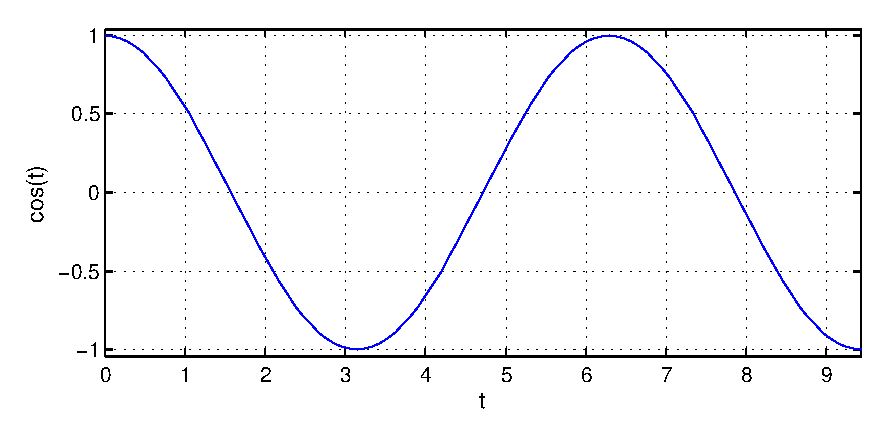
\includegraphics[width=0.495\textwidth]{\pwd/plots/example1}\label{fig:intro:floats:usage:figure-ex1}} \hfill
  \subfigure[right side]{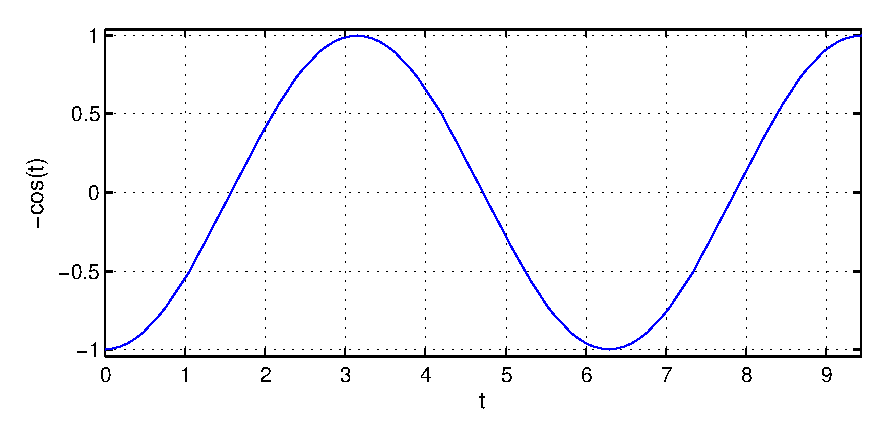
\includegraphics[width=0.495\textwidth]{\pwd/plots/example2}\label{fig:intro:floats:usage:figure-ex2}}
  \caption{Two subplots.}
  \label{fig:intro:floats:usage:figure}
\end{figure}

\noindent To create such two-column figures, the following simplified command can be used:
{
\scriptsize
\begin{verbatim}
  \twofigs{\pwd/plots/example1}{left side}{-ex1}{\pwd/plots/example2}{right side}{-ex2}{Two subplots.}{intro:floats:usage:figure-std}
\end{verbatim}
}
\noindent Reference it using:
\begin{verbatim}
\fref{fig:intro:floats:usage:figure-std}
\end{verbatim}

\noindent See \Fref{tab:intro:floats:figures} for more standardized commands. Captions and labels are mandatory for all these commands.
\begin{longtable}{>{\tiny}l|>{\tiny}p{0.3\textwidth}}
  \normalsize\textbf{Command} & \normalsize\textbf{Description} \\\hline
  \verb|\fig{file}{caption}{label}| & Standard figure, full textwidth. \\\hline
  \verb|\figc{param}{file}{caption}{label}| & Standard figure with controllable parameters for includegraphics. \\\hline
  \verb|\twofig{file_l}{caption_l}{file_r}{caption_r}{caption}{label}| & Two figures, side by side. \\\hline
  \verb|\twofigs{file_l}{caption_l}{add.label_l}{filename_r}{caption_r}{add.label_l}{caption}{label}| & Two figures, side by side, with labels for each subfigure.\\\hline
  \verb|\twofigc{param_l}{file_l}{caption_l}{param_l}{filename_r}{caption_r}{caption}{label}| & Two figures, side by side, with controllable parameters for includegraphics. \\\hline
  \verb|\figf|, \verb|\figcf|, \verb|\twofigf|, \verb|\twofigsf|, \verb|\twofigcf| & Like the above, but with framed figures. \\
  \caption{Standardized commands for figures.}
  \label{tab:intro:floats:figures}
\end{longtable}


% **************************************************************************************************
\newsubsection{Listings}{intro:floats:listings}

A code listing can be included from an external file using:

\begin{verbatim}
\filelisting{styMatlab}{\pwd/plots/matlab.m}{Some matlab code example.}{code-example}
\end{verbatim}

\noindent which looks like this:

\filelisting{styMatlab}{\pwd/plots/matlab.m}{Some matlab code example.}{code-example}

\vspace{5mm}
\noindent To include only certain lines of an external file you can supply option parameters to the listing command like this:

\begin{verbatim}
\filelisting[firstline=3, lastline=6]{styMatlab}{\pwd/plots/matlab.m}{Subset printed.}{param-example}
\end{verbatim}

\vspace{5mm}
\noindent A reference to \Fref{lst:code-example} can be created using

\begin{verbatim}
\Fref{lst:code-example}
\end{verbatim}

\vspace{5mm}
\noindent You can also write code inline using:

\begin{verbatim}
\begin{lstlisting}[style=styMatlab,caption={Some fancy matlab inline code},label={lst:matlabInline}]
clf;
plot(sin(0:1:5));
\end{lstlisting}
\end{verbatim}
